\documentclass{beamer}
\usepackage{amsmath}
\usepackage{amssymb}

\mode<presentation>
{
  \usetheme{Warsaw}
  % or ...

  \setbeamercovered{transparent}
  % or whatever (possibly just delete it)
}

\usepackage[english]{babel}
% or whatever

\usepackage[latin1]{inputenc}
% or whatever

\usepackage{times}
\usepackage[T1]{fontenc}
% Or whatever. Note that the encoding and the font should match. If T1
% does not look nice, try deleting the line with the fontenc.

\usepackage{amsmath}
\title[Network Traffic Classification] % (optional, use only with long paper titles)
{Network Traffic Classification}

\subtitle
{Naive Bayes Classification}

\author % (optional, use only with lots of authors)
{Kefei Lu}
% - Use the \inst{?} command only if the authors have different
%   affiliation.

\institute[Universities of Miami] % (optional, but mostly needed)
{
  Department of Electrical and Computer Engineering\\
  University of Miami}
% - Use the \inst command only if there are several affiliations.
% - Keep it simple, no one is interested in your street address.

\date[] % (optional)
{2009-11-24}

\subject{}
% This is only inserted into the PDF information catalog. Can be left
% out. 

% Delete this, if you do not want the table of contents to pop up at
% the beginning of each subsection:
\AtBeginSubsection[]
{
  \begin{frame}<beamer>{Outline}
    \tableofcontents[currentsection,currentsubsection]
  \end{frame}
}

\begin{document}
\begin{frame}
  \titlepage
\end{frame}

\begin{frame}{Outline}
  \tableofcontents
  % You might wish to add the option [pausesections]
\end{frame}

\begin{frame}{The System Flow Chart}
	\begin{figure}[tbp]
	    \centering
	    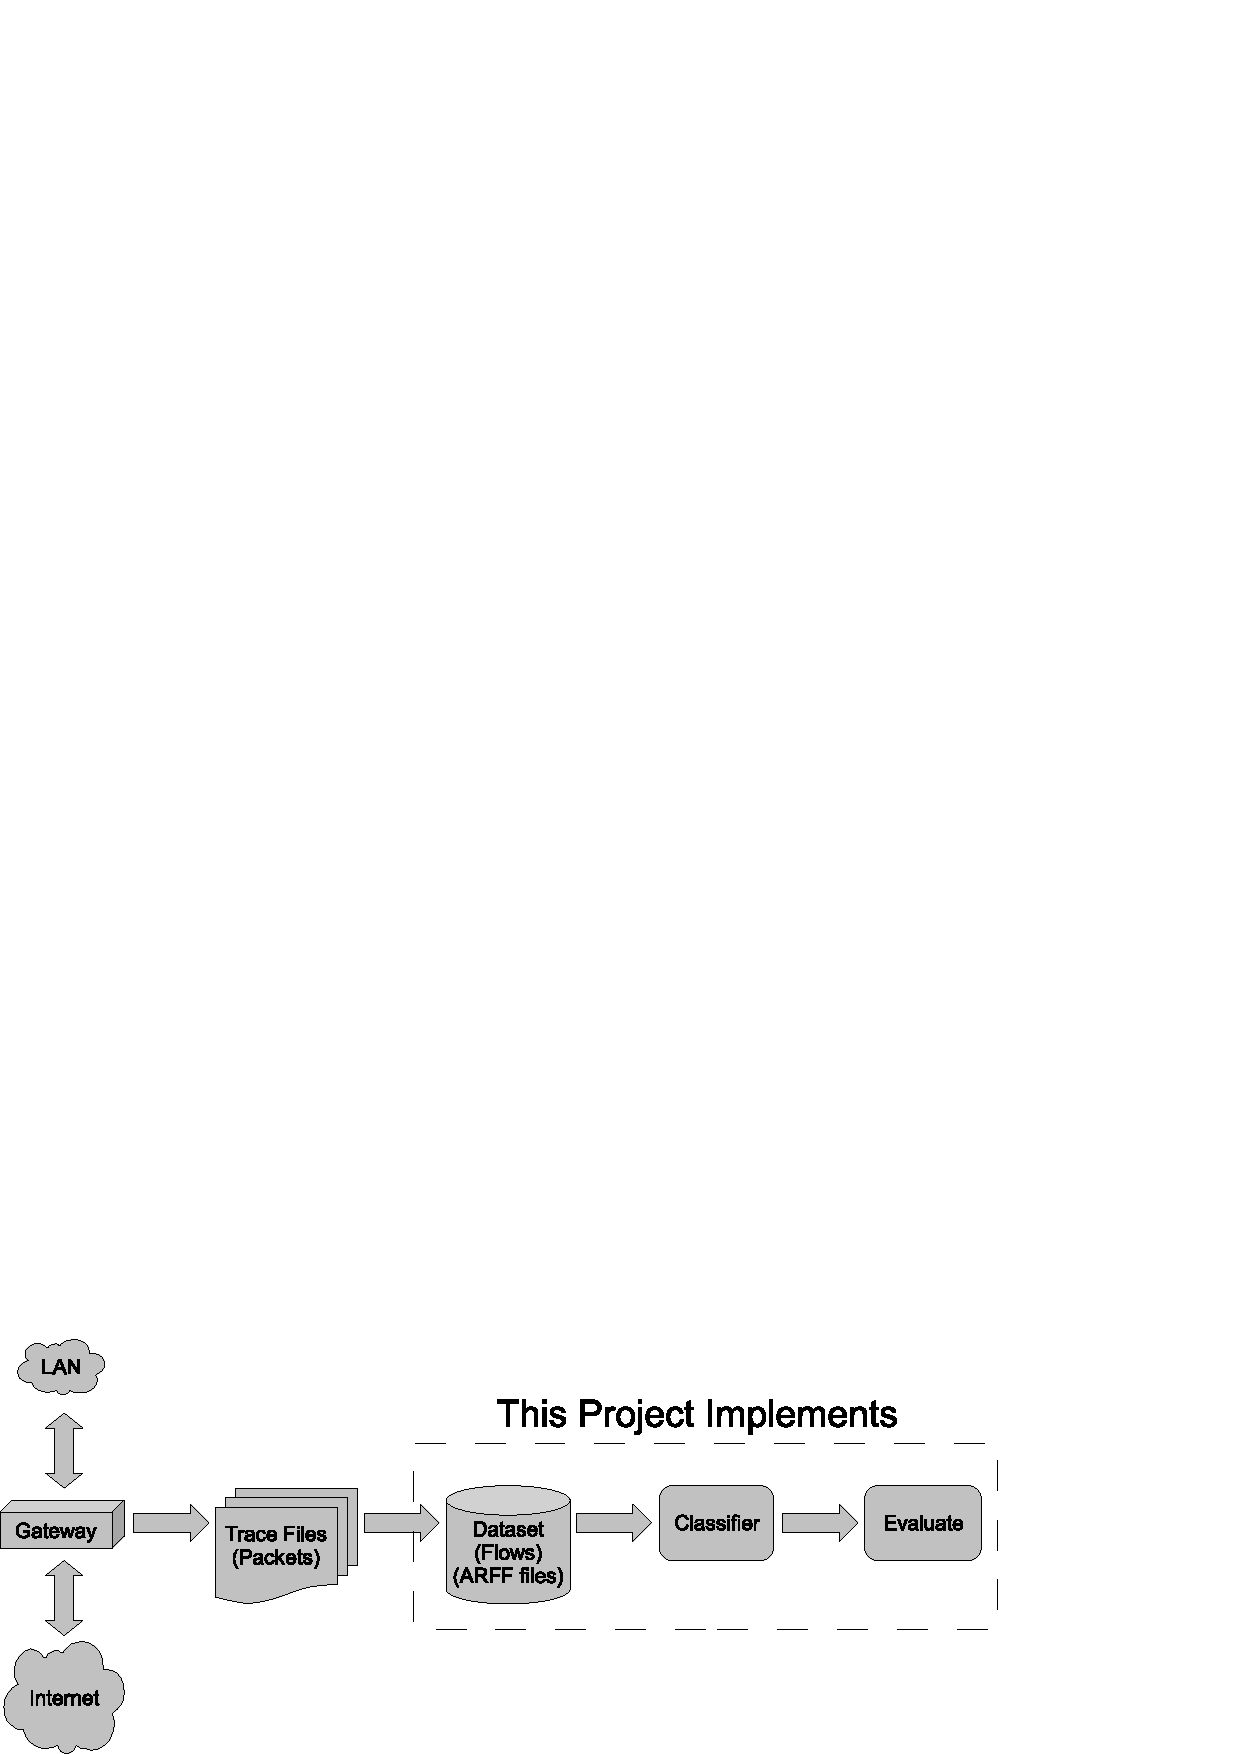
\includegraphics[width=0.9\textwidth]{pic/flow_chart.png}
	    \caption{The flow chart of network traffic classification.}
	    \label{fig:flow_chart}
	\end{figure}
\end{frame}

\begin{frame}{The Implemented Structure}
	\begin{figure}[tbp]
	    \centering
	    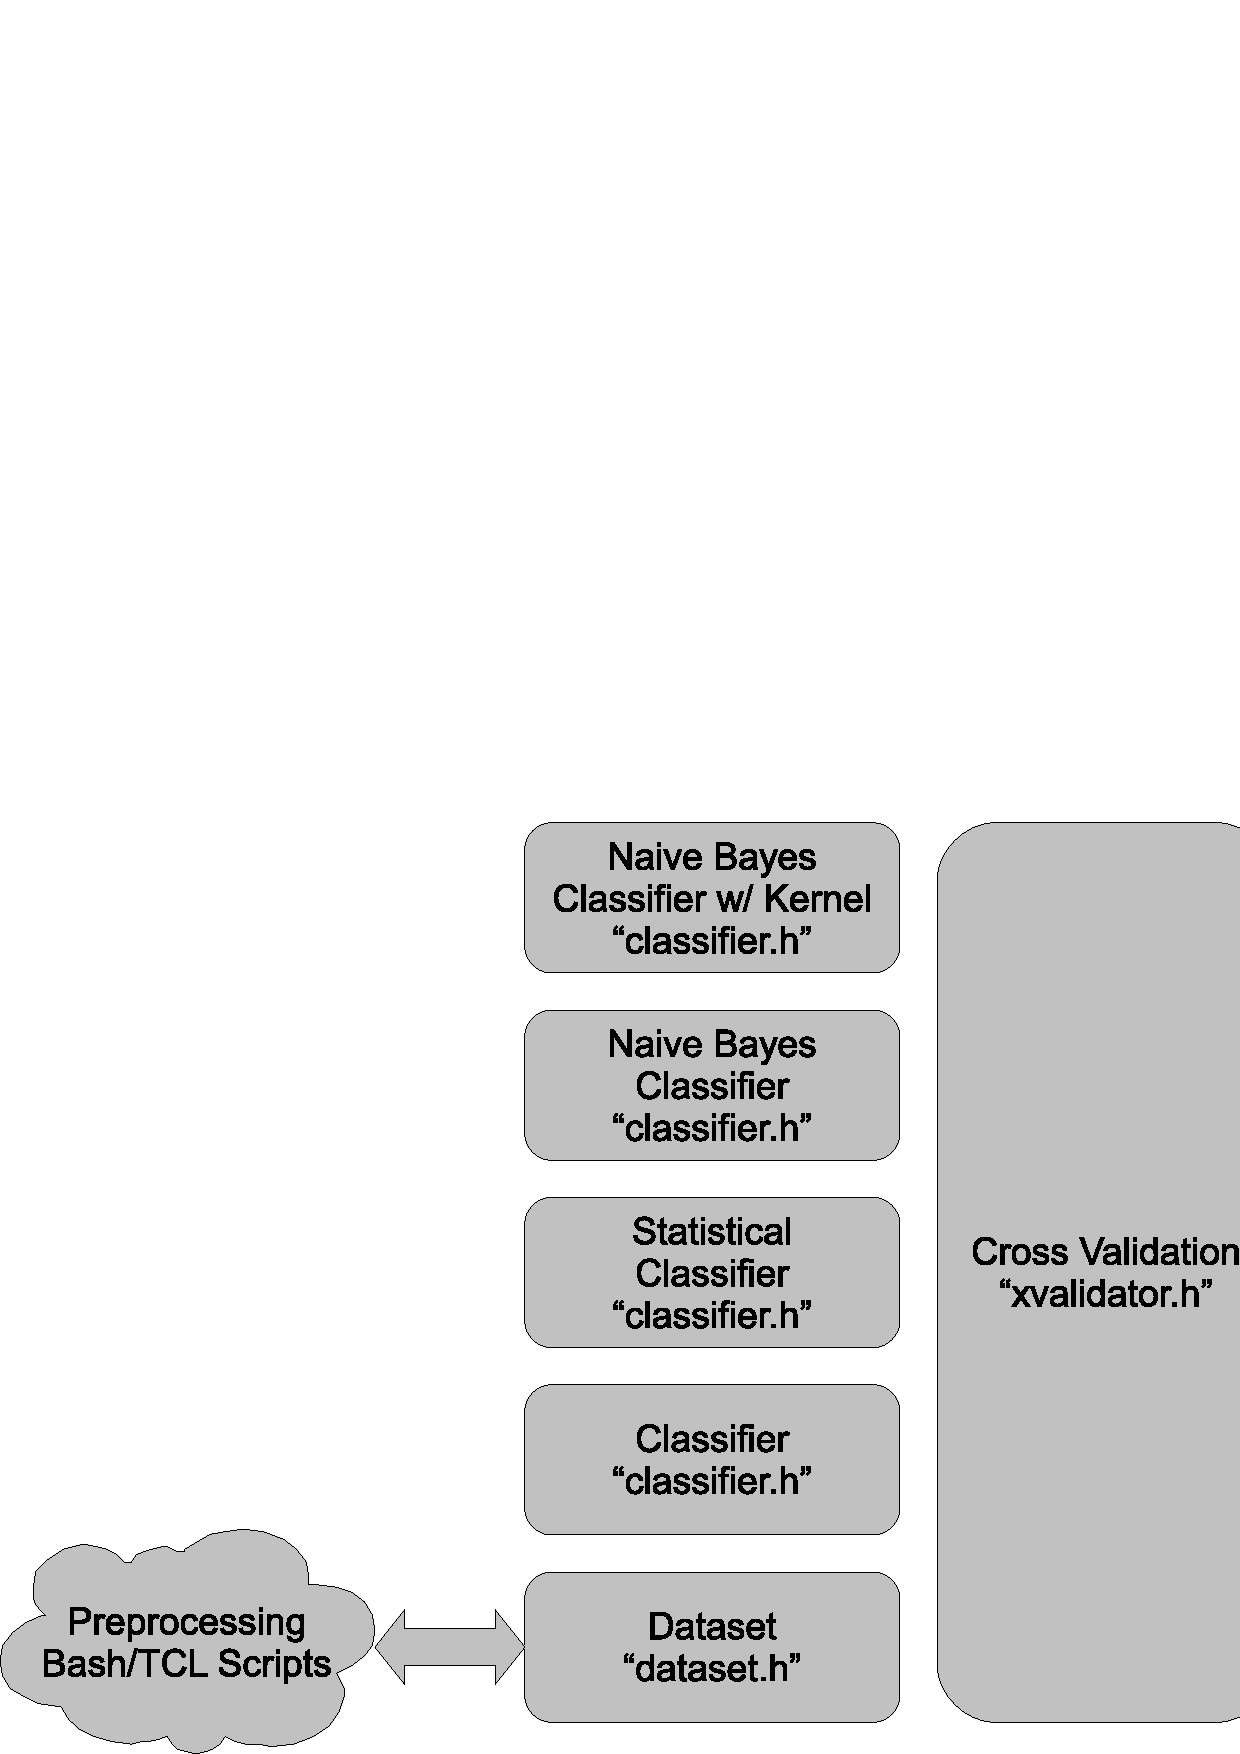
\includegraphics[width=0.9\textwidth]{pic/struct.png}
	    \caption{The Implemented Structure}
	    \label{fig:flow_chart}
	\end{figure}
\end{frame}

\begin{frame}{The Naive Bayes Method}

\end{frame}

\begin{frame}
\end{frame}

\begin{frame}
\end{frame}
\end{document}
